% Created 2021-02-16 Tue 12:43
% Intended LaTeX compiler: pdflatex
\documentclass[english]{article}
  \usepackage[T1, T2A]{fontenc}
\usepackage[lutf8]{luainputenc}
\usepackage[english, russian]{babel}
\usepackage{minted}
\usepackage{graphicx}
\usepackage{longtable}
\usepackage{hyperref}
\usepackage{xcolor}
\usepackage{natbib}
\usepackage{amssymb}
\usepackage{amsmath}
\usepackage{caption}
\usepackage{mathtools}
\usepackage{amsthm}
\usepackage{tikz}
\usepackage{grffile}
\usepackage{extarrows}
\usepackage{wrapfig}
\usepackage{rotating}
\usepackage{placeins}
\usepackage[normalem]{ulem}
\usepackage{amsmath}
\usepackage{textcomp}
\usepackage{capt-of}
  
  \usepackage{geometry}
  \geometry{a4paper,left=2.5cm,top=2cm,right=2.5cm,bottom=2cm,marginparsep=7pt, marginparwidth=.6in}

   \usepackage{hyperref}
   \hypersetup{
       colorlinks=true,
       linkcolor=blue,
       filecolor=orange,
       citecolor=black,      
       urlcolor=cyan,
       }

  \usetikzlibrary{decorations.markings}
  \usetikzlibrary{cd}
  \usetikzlibrary{patterns}

  \newcommand\addtag{\refstepcounter{equation}\tag{\theequation}}
  \newcommand{\eqrefoffset}[1]{\addtocounter{equation}{-#1}(\arabic{equation}\addtocounter{equation}{#1})}


  \newcommand{\R}{\mathbb{R}}
  \renewcommand{\C}{\mathbb{C}}
  \newcommand{\N}{\mathbb{N}}
  \newcommand{\rank}{\text{rank}}
  \newcommand{\const}{\text{const}}
  \newcommand{\grad}{\text{grad}}

  \theoremstyle{plain}
  \newtheorem{axiom}{Аксиома}
  \newtheorem{lemma}{Лемма}
  \newtheorem{manuallemmainner}{Лемма}
  \newenvironment{manuallemma}[1]{%
    \renewcommand\themanuallemmainner{#1}%
    \manuallemmainner
  }{\endmanuallemmainner}

  \theoremstyle{remark}
  \newtheorem*{remark}{Примечание}
  \newtheorem*{solution}{Решение}
  \newtheorem{corollary}{Следствие}[theorem]
  \newtheorem*{examp}{Пример}
  \newtheorem*{observation}{Наблюдение}

  \theoremstyle{definition}
  \newtheorem{task}{Задача}
  \newtheorem{theorem}{Теорема}[section]
  \newtheorem*{definition}{Определение}
  \newtheorem*{symb}{Обозначение}
  \newtheorem{manualtheoreminner}{Теорема}
  \newenvironment{manualtheorem}[1]{%
    \renewcommand\themanualtheoreminner{#1}%
    \manualtheoreminner
  }{\endmanualtheoreminner}
  \captionsetup{justification=centering,margin=2cm}
  \newenvironment{colored}[1]{\color{#1}}{}

  \tikzset{->-/.style={decoration={
    markings,
    mark=at position .5 with {\arrow{>}}},postaction={decorate}}}
  \makeatletter
  \newcommand*{\relrelbarsep}{.386ex}
  \newcommand*{\relrelbar}{%
    \mathrel{%
      \mathpalette\@relrelbar\relrelbarsep
    }%
  }
  \newcommand*{\@relrelbar}[2]{%
    \raise#2\hbox to 0pt{$\m@th#1\relbar$\hss}%
    \lower#2\hbox{$\m@th#1\relbar$}%
  }
  \providecommand*{\rightrightarrowsfill@}{%
    \arrowfill@\relrelbar\relrelbar\rightrightarrows
  }
  \providecommand*{\leftleftarrowsfill@}{%
    \arrowfill@\leftleftarrows\relrelbar\relrelbar
  }
  \providecommand*{\xrightrightarrows}[2][]{%
    \ext@arrow 0359\rightrightarrowsfill@{#1}{#2}%
  }
  \providecommand*{\xleftleftarrows}[2][]{%
    \ext@arrow 3095\leftleftarrowsfill@{#1}{#2}%
  }
  \makeatother
\author{Ilya Yaroshevskiy}
\date{\today}
\title{Практика 2}
\hypersetup{
 pdfauthor={Ilya Yaroshevskiy},
 pdftitle={Практика 2},
 pdfkeywords={},
 pdfsubject={},
 pdfcreator={Emacs 28.0.50 (Org mode )}, 
 pdflang={English}}
\begin{document}

\maketitle
\tableofcontents

\begin{task}
Трамваи ходят с интервалом строго 15 мин.
Вероятность того что придя на остановку придется ждать не более пяти минут.
\end{task}

\begin{task}
Параллельно на прямой расставляются мины с интервалом 10 меторв. Найти
вероятность того что танк шириной 3 метра подорвется на мине.
\end{task}
\begin{solution}
\-
\begin{center}
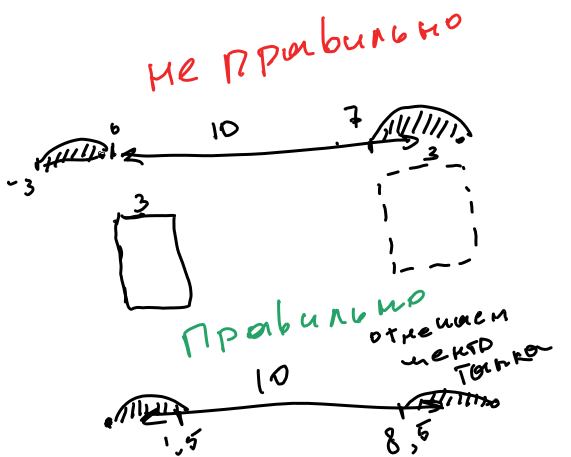
\includegraphics[scale=0.5]{2_1.png}
\end{center}
Отмечаем центр танка.
\[ \frac{3}{10} \]
\end{solution}
\begin{task}
Двое человек договорились встретиться между 12 и 13 часами дня. Найти
веротяность того что один из них не будет ждать другово больше 15 мин.
\end{task}
\begin{solution}
\-
\begin{center}
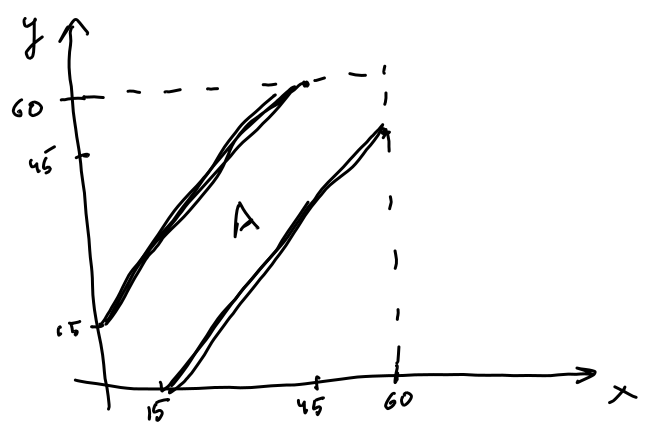
\includegraphics[scale=0.3]{2_2.png}
\end{center}
\begin{itemize}
\item \(x\) --- время приходя первого
\item \(y\) --- время прихода второго
\end{itemize}
\[ |x - y| \le 15 \]
\[ -15 \le x - y \le 15 \]
\begin{enumerate}
\item \[ y \le x + 15 \]
\begin{center}
\begin{tabular}{lrr}
\(x\) & 0 & 45\\
\(y\) & 15 & 60\\
\end{tabular}
\end{center}
\item \[ y \ge x - 15 \]
\begin{center}
\begin{tabular}{lrr}
\(x\) & 15 & 60\\
\(y\) & 0 & 45\\
\end{tabular}
\end{center}
\end{enumerate}
\[ S(\Omega) = 60^2 \]
\[ S(A) = 60^2 - 2\cdot45^2\cdot\frac{1}{2} \]
\[ P(A) = \frac{15\cdot105}{60^2} = \frac{7}{16} \]
\end{solution}
\begin{task}
В круге радиуса \textbf{1} наугад нарисовали хорду. Найти веротяность того
что ее длина будет больше стороны вписаного правильного треугольника
\end{task}
\begin{solution}
\begin{center}
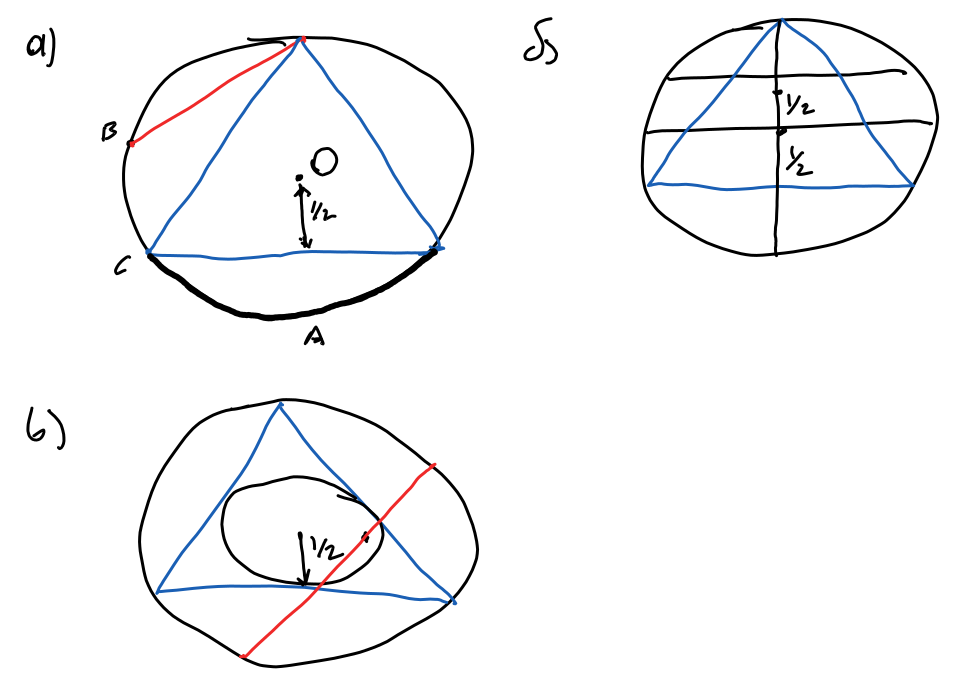
\includegraphics[width=.9\linewidth]{2_3.png}
\end{center}
\begin{enumerate}
\item \[ P(A) = \frac{1}{3} \]
\item \[ P(A) = \frac{1}{2} \]
\item \[ S(\Omega) = \pi\cdot1^2 = \pi \]
\[ S(A) = \pi \cdot \left(\frac{1}{2}\right)^2 = \frac{\pi}{4} \]
\[ P(A) = \frac{1}{4} \]
\end{enumerate}
\end{solution}
\end{document}
